\section{Introducción}\label{sec:introduccion}

\begin{frame}{Simulación de Multitudes}
    \begin{center}
        \begin{minipage}[c]{0.6\textwidth}
            \begin{block}{Características}
                \begin{itemize}
                    \item N personas moviéndose en un espacio.
                    \item Cada persona tiene definida su posición, velocidad y radio.
                    \item Las personas desean moverse a una posición objetivo y con una velocidad deseada, $v_d$.
                    \item Las personas desean evitar colisiones entre ellas.
                    \item Las personas viajan en línea recta y a velocidad constante entre instantes de tiempo.
                \end{itemize}
            \end{block}
        \end{minipage}
        \hfill
        \begin{minipage}[c]{0.3\textwidth}
            \begin{figure}
                \centering
                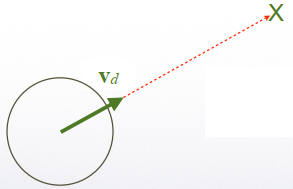
\includegraphics[width=\textwidth]{pic/01-introduccion/particle-vd}
                \label{fig:particle-vd}
            \end{figure}
        \end{minipage}
    \end{center}
\end{frame}

\begin{frame}{Simulación de Multitudes}
    \begin{block}{Regímenes}
        \begin{itemize}
            \item \textbf{Condiciones cooperativas}
            \begin{itemize}
                \item Prevalece el respeto, la caballerosidad y otros valores sociales.
                \item El contacto físico es prácticamente nulo.
                \item Las densidades son bajas o moderadas.
            \end{itemize}
            \item \textbf{Condiciones competitivas}
            \begin{itemize}
                \item Prevalece la competencia, la supervivencia y otros valores individuales.
                \item El contacto físico es frecuente.
                \item Las densidades y presiones son altas.
            \end{itemize}
        \end{itemize}
    \end{block}
\end{frame}

\begin{frame}{Modelo}
    \textbf{\large{Contractile Particle Model (CPM)}}
    \begin{center}
        \begin{minipage}[c]{0.6\textwidth}
            \begin{block}{Características}
                \begin{itemize}
                    \item Las personas tienen un radio variable, $r \in [r_{min}, r_{max}]$.
                    \item La velocidad deseada depende del radio de la persona.
                    \item Ante el contacto, el radio de las personas se contrae al mínimo y aparece una velocidad de escape $v_e$.
                \end{itemize}
            \end{block}
        \end{minipage}
        \hfill
        \begin{minipage}[c]{0.3\textwidth}
            \begin{figure}
                \centering
                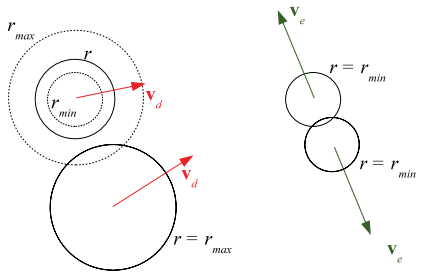
\includegraphics[width=\textwidth]{pic/01-introduccion/cpm}
                \label{fig:cpm}
            \end{figure}
        \end{minipage}
    \end{center}
\end{frame}

\begin{frame}{Modelo}
    \textbf{\large{Contractile Particle Model (CPM)}}
    \begin{block}{Velocidad deseada}
        \begin{equation*}
            v_d^i = v_{d\ max} \left[ \frac{(r^i - r_{min})}{(r_{max} - r_{min})} \right]^{\beta}
        \end{equation*}
    \end{block}
    \begin{block}{Salto de instante}
        \begin{equation*}
            \Delta t = \frac{r_{min}}{2 \max (v_{d\ max}, v_e)}
        \end{equation*}
    \end{block}
\end{frame}

\begin{frame}{Modelo}
    \textbf{\large{Contractile Particle Model (CPM)}}
    \begin{block}{Velocidad}
        \begin{equation*}
            \mathbf{v}^i = \begin{cases}
                \mathbf{v}_d^i & \text{si $p^i$ está libre de contacto} \\
                \mathbf{v}_e & \text{sino}
            \end{cases}
        \end{equation*}
    \end{block}
    \begin{block}{Diferencial de radio}
        \begin{equation*}
            \Delta r = \frac{r_{max}}{\left( \frac{\tau}{\Delta t} \right)}
        \end{equation*}
    \end{block}
\end{frame}



